\documentclass[a4paper,12pt]{article}

\usepackage[czech]{babel}
\usepackage[utf8]{inputenc}

\usepackage{graphicx}	%kvůli eps souboru z MATLABu
\usepackage{amsmath}	%matice
\usepackage{float}		%obrázky
\usepackage{subcaption} %obrázky vedle sebe

\newcommand{\tg}{\mathop{\mathrm{tg}}}
\newcommand{\arctg}{\mathop{\mathrm{arctg}}}

\title{Zpráva laboratorní úloze}
\author{Matouš Vrba, Tomáš Glabazňa}
\date{\today}

% === Formát stránky ===
\usepackage[a4paper]{geometry}
\geometry{
	verbose,
	tmargin=2.2cm,
	bmargin=1.5cm,
	lmargin=1.5cm,
	rmargin=1.5cm}

\begin{document}

\maketitle
\pagebreak

\section{Regulátor úhlu natočení kyvadla}
Regulátor pro kyvadlo jsme navrhovali tak, aby co nejrychleji a s co nejmenším překmitem reguloval polohu kyvadla vždy do spodní polohy, tedy na hodnotu $\varphi_p=-90^{\circ}=-\frac{\pi}{2}$. Každý regulátor jsme vždy nejdříve navrhli nějakou metodou na linearizovaném systému v pracovním bodě $\mathbf{x_0} = \left[\varphi_{m0}, \varphi_{p0}, \dot{\varphi}_{m0}, \dot{\varphi}_{p0}\right] = \left[0, -\frac{\pi}{2}, 0, 0\right]$, potom jsme ho vyzkoušeli na linearizovaném a nelineárním modelu a zkontrolovali jsme, že se chová rozumně - především jsme kontrolovali, že vstupní saturace systému nepokazí odezvy. Až pokud regulátor obstál na linearizovaném i nelineárním modelu, vyzkoušeli jsme ho na reálném systému. Zapojení pro testování regulátorů na následujícím obrázku:
\begin{figure}[H]
	\centering
    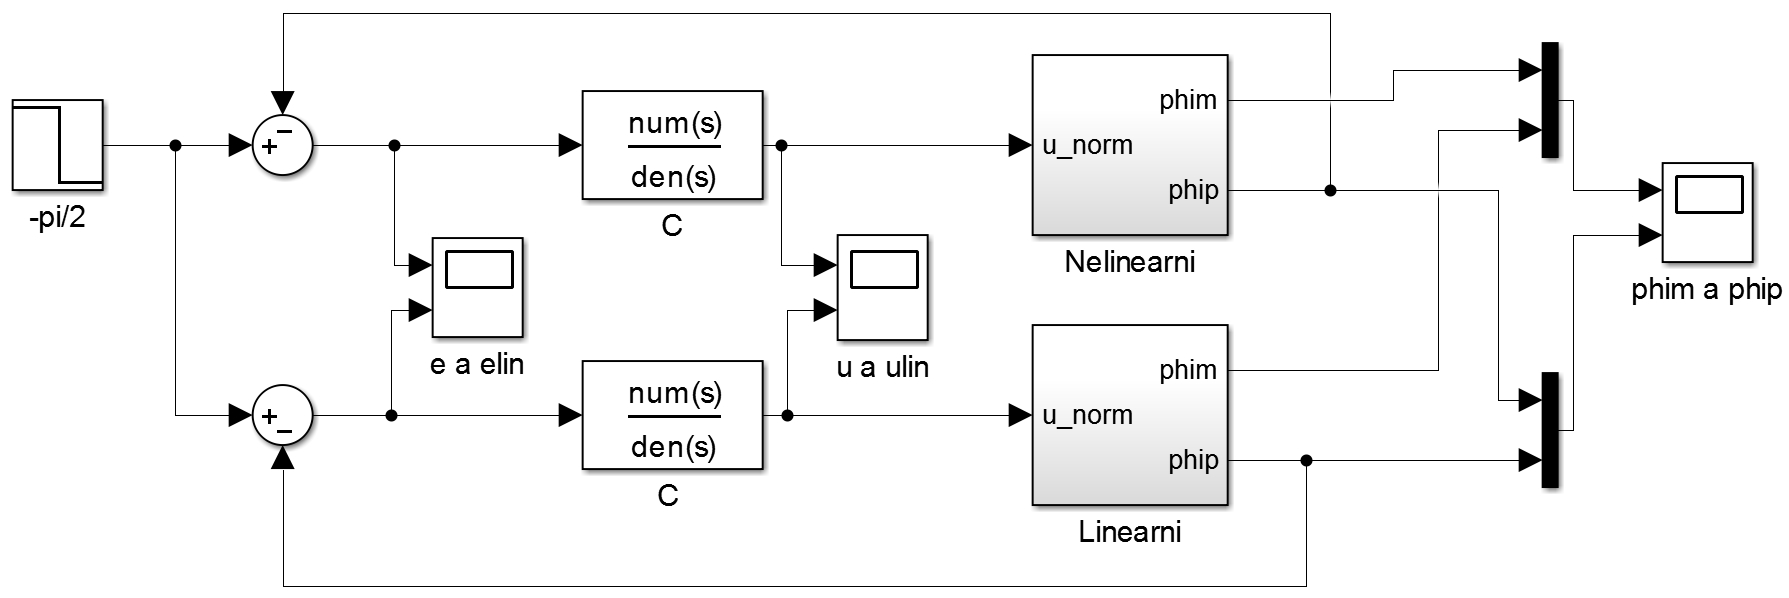
\includegraphics[scale=0.25]{schema_rizeni_nanecisto}
    \caption{Testovací zapojení regulátorů}
\end{figure}

\subsection{Obecný regulátor, navržený polynomiálními metodami}
Tento regulátor jsme navrhovali polynomiálními metodami. Nejdříve jsme si rozumně určili polohy, do kterých bychom chtěli posunout póly výsledného systému a sestavili charakteristický polynom $c(s)$ pro tyto póly. Potom jsme dosadili do rovnice pro charakteristický polynom výsledného systému se zapojeným regulátorem, kde regulátor $C = \frac{y(s)}{x(s)}$ a soustava $G = \frac{b(s)}{a(s)}$, a tuto rovnici se dvěma neznámými polynomy $y$ a $x$ vyřešili pomocí funkce Polynomial Toolboxu \textit{axbyc} s parametrem \textit{"miny"}:
\begin{align*}
c(s) &= (s + 12) (s + 5 - 10j) (s + 5 + 10j) (s + 20)^2	\\
b(s)\cdot y(s) + a(s)\cdot x(s) &= c(s)	\\
-18,1s\cdot y(s) + (s^3 + 7,021s^2 + 74,37s + 461)\cdot x(s) &=  (s + 12) (s + 5 - 10j) (s + 5 + 10j) (s + 20)^2
\end{align*}
Do žádaného charakteristického polynomu jsme museli přidat dva póly ($(s+20)^2$), aby měla tato rovnice řešení, které vede na ryzí regulátor.
\newline
Výsledný přenos regulátoru:
\begin{align*}
C = \frac{13,09s^2 - 354,3s - 1981}{16s^2 + 879,7 + 20820}
\end{align*}
Příklad odezvy kyvadla s tímto regulátorem na poruchu je na grafech na další stránce. Z grafů je vidět, že kyvadlo se neustaluje na nulové odchylce, což je způsobeno chybou enkoderových snímačů (nebo komunikace řídicího modulu s MATLABem), které někdy vynechávají kroky. Tato chyba se naintegruje a má za následek odchylku od reference, i když je kyvadlo už ve skutečnosti ustálené.
\newline
\newline
Až na tuto chybu ale regulátor funguje velmi dobře a kyvadlo stabilizuje vždy maximálně do dvou sekund.
\begin{figure}[H]
	\centering
    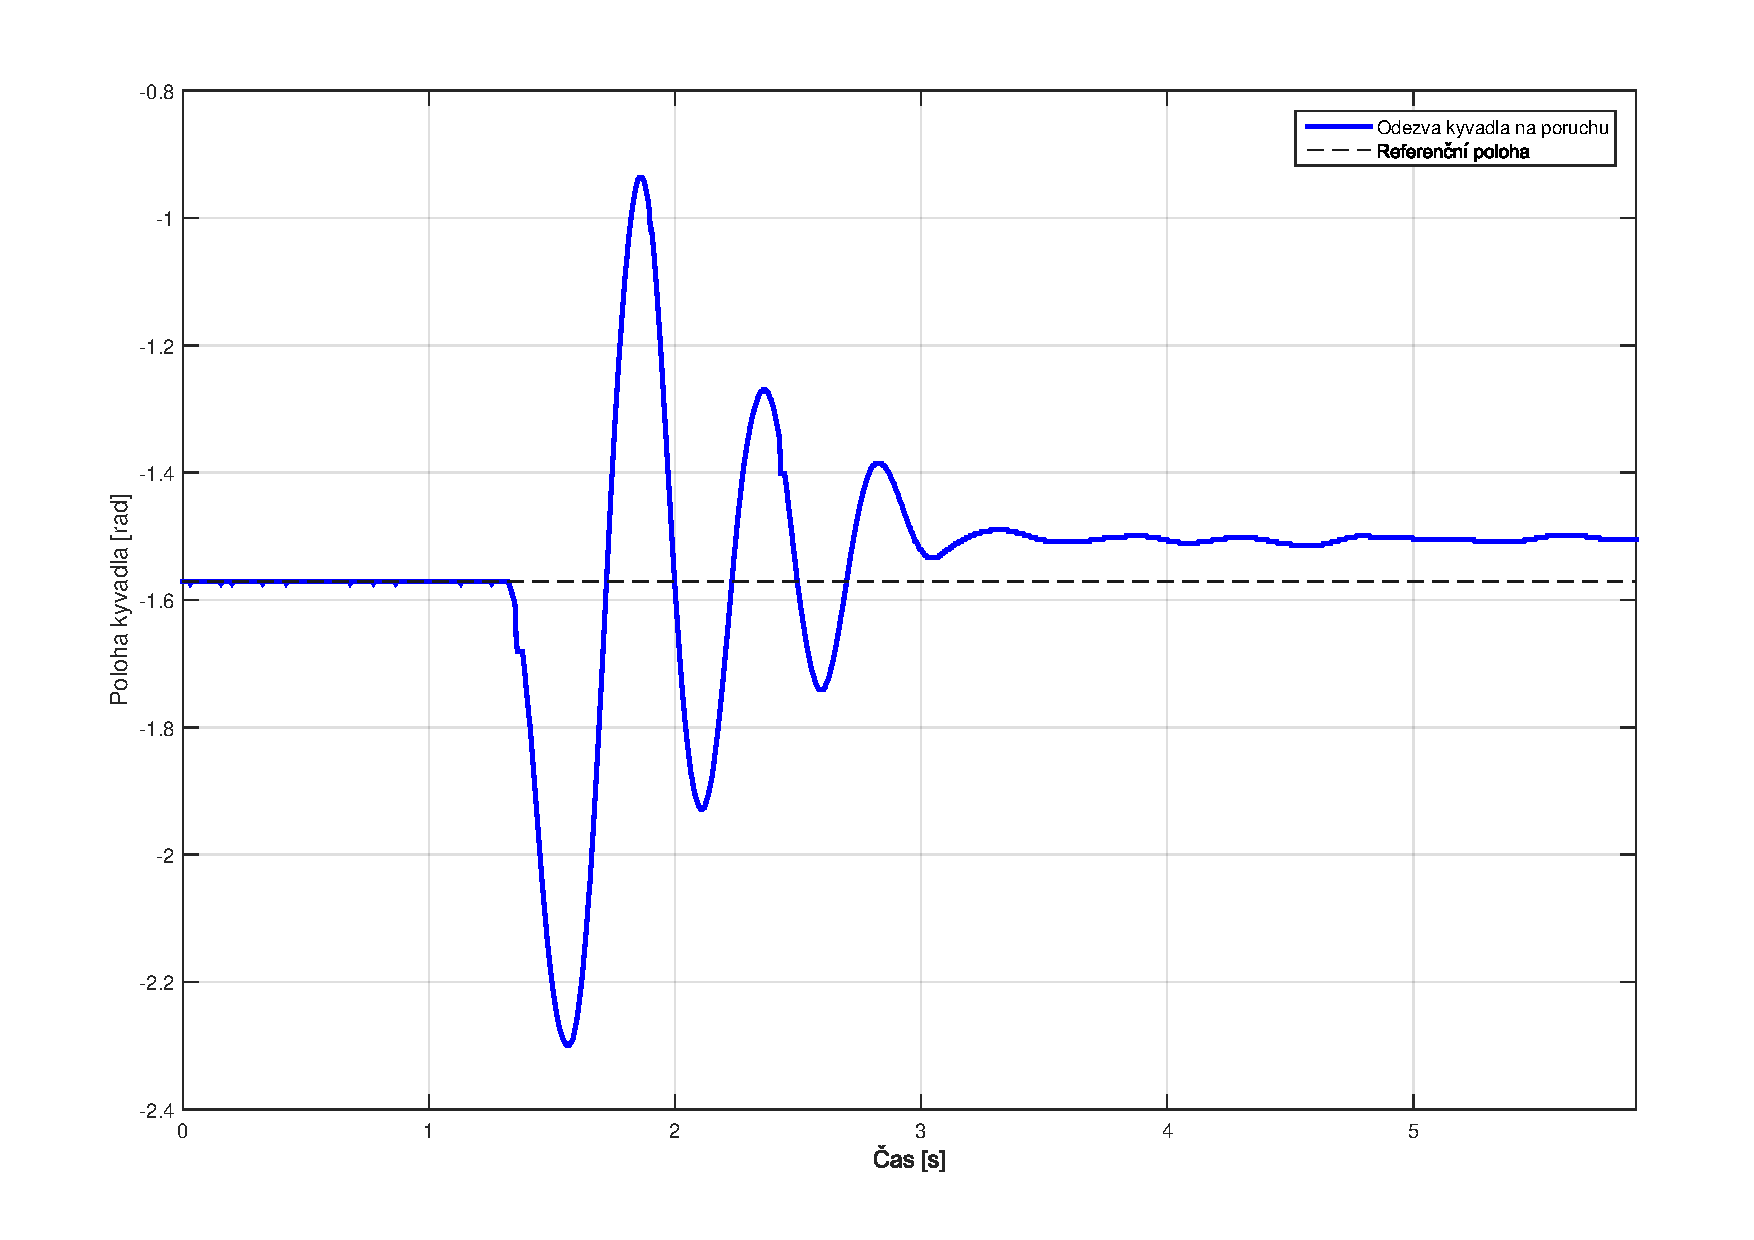
\includegraphics[scale=0.55]{odezva_kyvadlo_poly}
    \caption{Odezva kyvadla s polynomiálním regulátorem na poruchu}
\end{figure}
\begin{figure}[H]
	\centering
    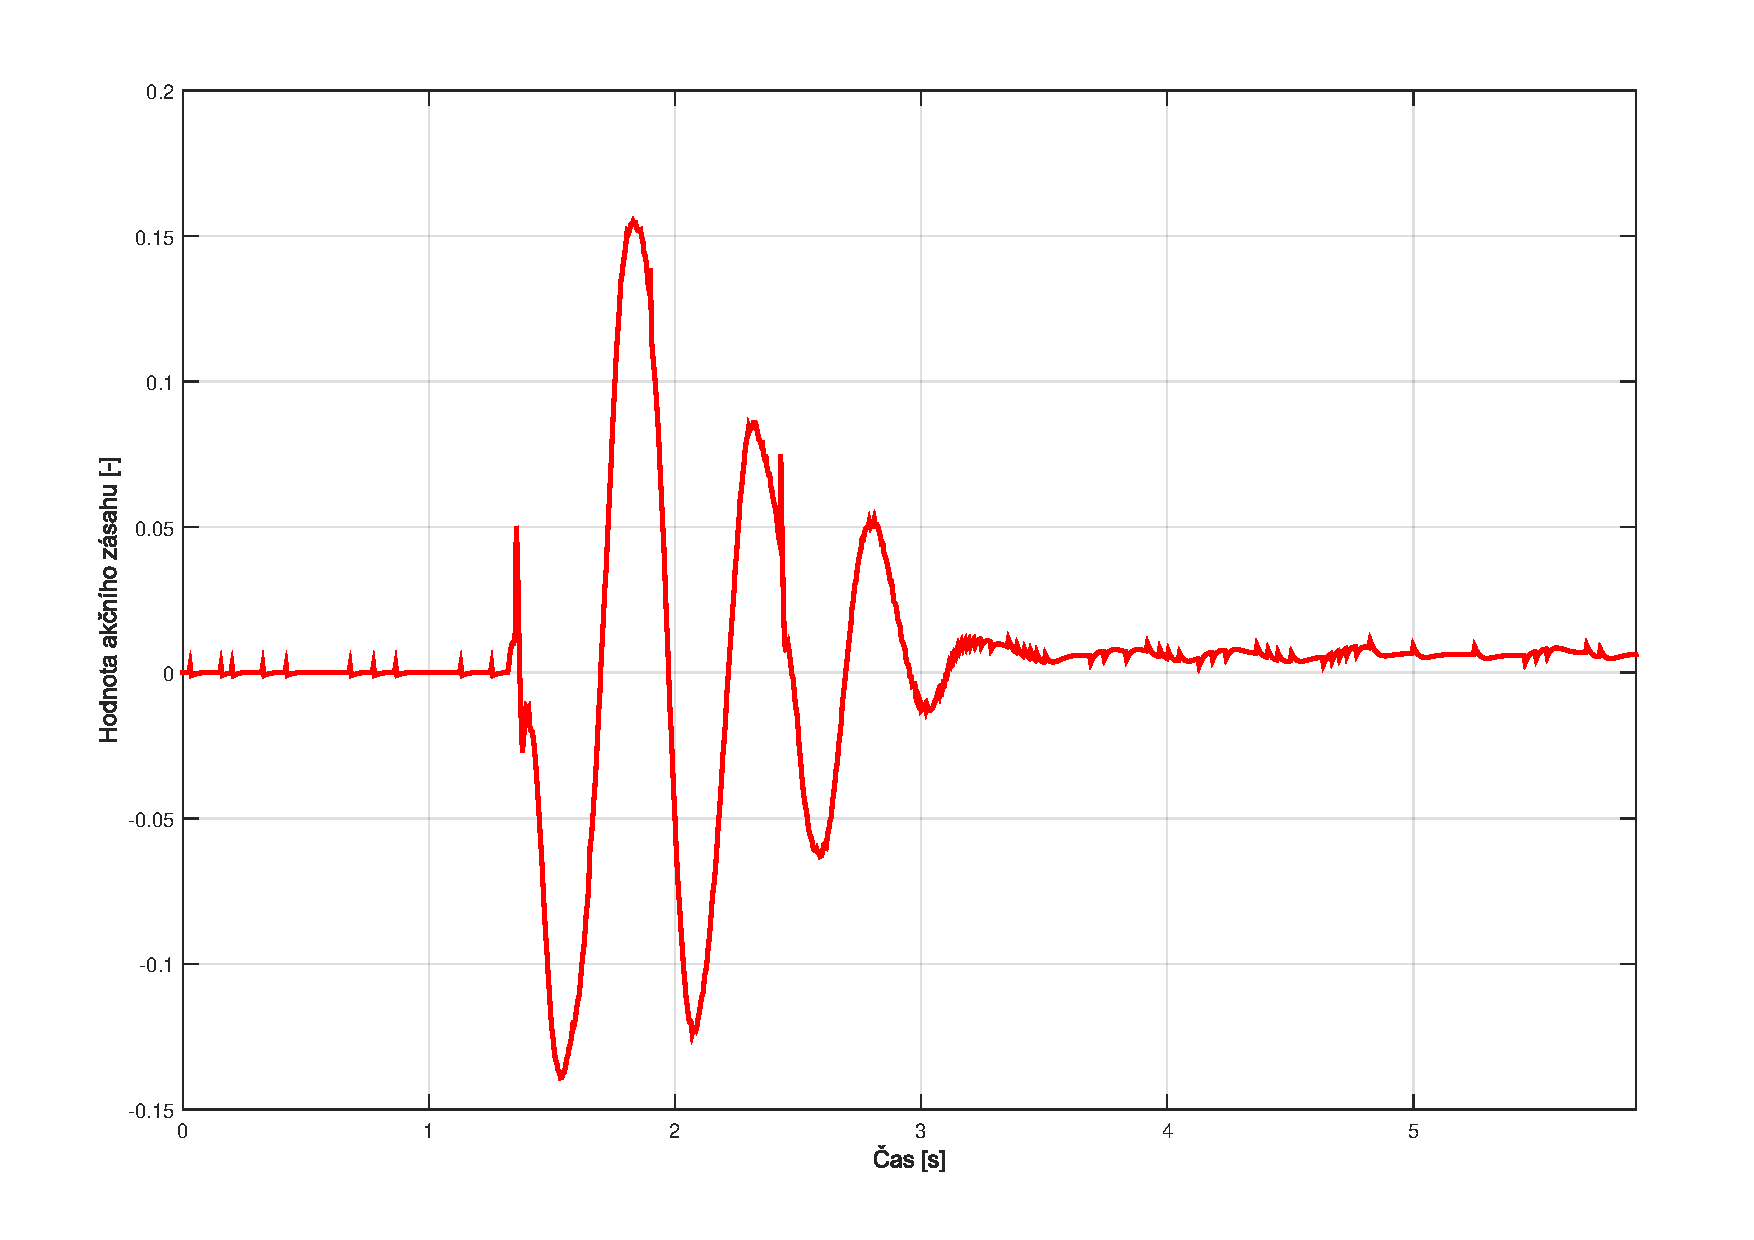
\includegraphics[scale=0.55]{odezva_kyvadlo_poly_akcnizasah}
    \caption{Akční zásah polynomiálního regulátoru}
\end{figure}


\subsection{PID regulátor, navržený root locusem}
Tento regulátor jsme navrhovali polynomiálními metodami. Nejdříve jsme si rozumně určili polohy, do kterých bychom chtěli posunout póly výsledného systému a sestavili charakteristický polynom $c(s)$ pro tyto póly. Potom jsme dosadili do rovnice pro charakteristický polynom výsledného systému se zapojeným regulátorem, kde regulátor $C = \frac{y(s)}{x(s)}$ a soustava $G = \frac{b(s)}{a(s)}$, a tuto rovnici se dvěma neznámými polynomy $y$ a $x$ vyřešili pomocí funkce Polynomial Toolboxu \textit{axbyc} s parametrem \textit{"miny"}:
\begin{align*}
c(s) &= (s + 12) (s + 5 - 10j) (s + 5 + 10j) (s + 20)^2	\\
b(s)\cdot y(s) + a(s)\cdot x(s) &= c(s)	\\
-18,1s\cdot y(s) + (s^3 + 7,021s^2 + 74,37s + 461)\cdot x(s) &=  (s + 12) (s + 5 - 10j) (s + 5 + 10j) (s + 20)^2
\end{align*}
Do žádaného charakteristického polynomu jsme museli přidat dva póly ($(s+20)^2$), aby měla tato rovnice řešení, které vede na ryzí regulátor.
\newline
Výsledný přenos regulátoru:
\begin{align*}
C = \frac{13,09s^2 - 354,3s - 1981}{16s^2 + 879,7 + 20820}
\end{align*}
Příklad odezvy kyvadla s tímto regulátorem na poruchu je na grafech na další stránce. Z grafů je vidět, že kyvadlo se neustaluje na nulové odchylce, což je způsobeno chybou enkoderových snímačů (nebo komunikace řídicího modulu s MATLABem), které někdy vynechávají kroky. Tato chyba se naintegruje a má za následek odchylku od reference, i když je kyvadlo už ve skutečnosti ustálené.
\newline
\newline
Až na tuto chybu ale regulátor funguje velmi dobře a kyvadlo stabilizuje vždy maximálně do dvou sekund.
\begin{figure}[H]
	\centering
    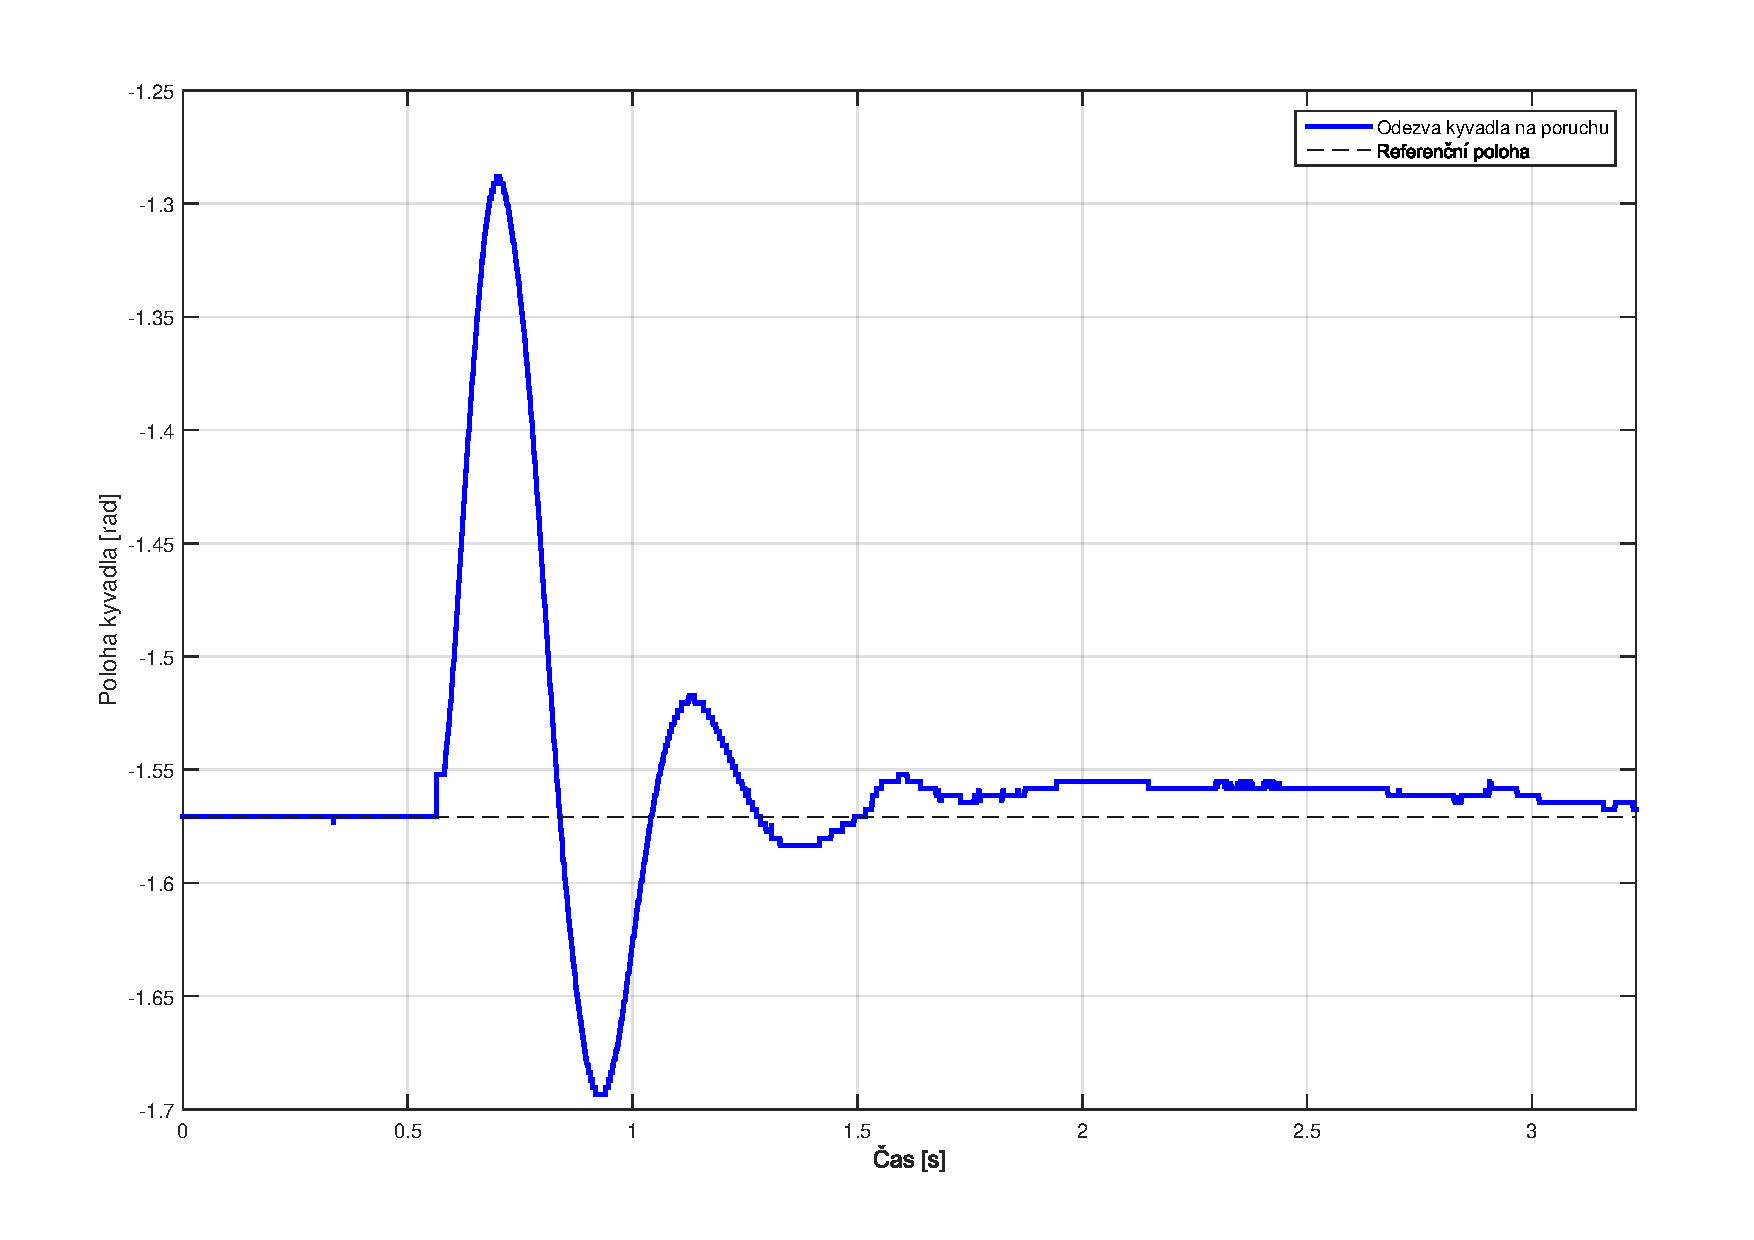
\includegraphics[scale=0.55]{odezva_kyvadlo_PID}
    \caption{Odezva kyvadla s PID regulátorem na poruchu}
\end{figure}
\begin{figure}[H]
	\centering
    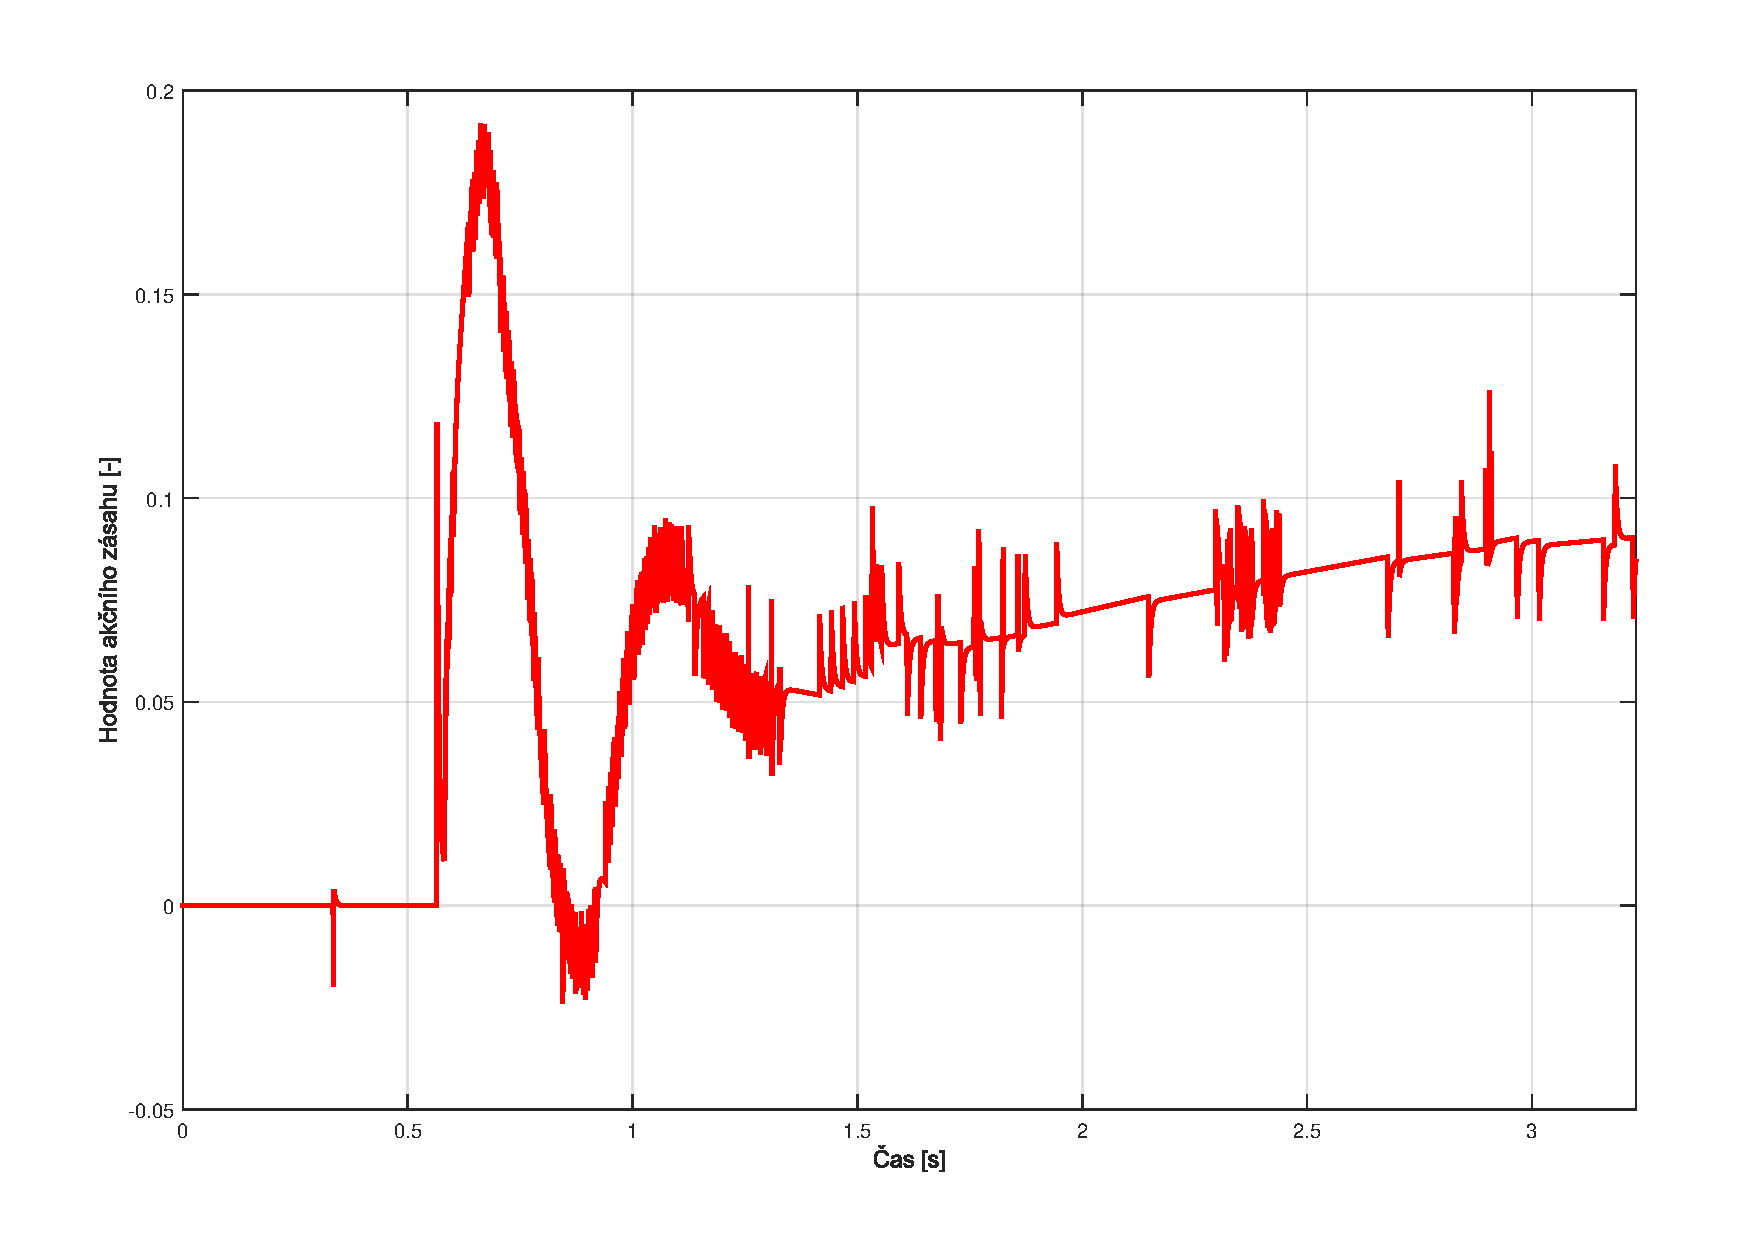
\includegraphics[scale=0.55]{odezva_kyvadlo_PID_akcnizasah}
    \caption{Akční zásah PID regulátoru}
\end{figure}



\end{document}